\iffalse
This file is protected by Copyright. Please refer to the COPYRIGHT file
distributed with this source distribution.

This file is part of OpenCPI <http://www.opencpi.org>

OpenCPI is free software: you can redistribute it and/or modify it under the
terms of the GNU Lesser General Public License as published by the Free Software
Foundation, either version 3 of the License, or (at your option) any later
version.

OpenCPI is distributed in the hope that it will be useful, but WITHOUT ANY
WARRANTY; without even the implied warranty of MERCHANTABILITY or FITNESS FOR A
PARTICULAR PURPOSE. See the GNU Lesser General Public License for more details.

You should have received a copy of the GNU Lesser General Public License along
with this program. If not, see <http://www.gnu.org/licenses/>.
\fi

%----------------------------------------------------------------------------------------
% Update the docTitle and docVersion per document
%----------------------------------------------------------------------------------------
\def\docTitle{OpenCPI\\ Matchstiq-Z1 BSP Case Study}
\def\docVersion{1.5}
%----------------------------------------------------------------------------------------
\def\snippetpath{../../../../../../doc/av/tex/snippets}
% Usage:
% \def\snippetpath{../../../../../doc/av/tex/snippets/}
% % Usage:
% \def\snippetpath{../../../../../doc/av/tex/snippets/}
% % Usage:
% \def\snippetpath{../../../../../doc/av/tex/snippets/}
% \input{\snippetpath/includes}
% From then on, you can use "input" With no paths to get to "snippets"
% You also get all "major" snippets not part of the global LaTeX_Header
% NOTE: If not using the global LaTeX_Header, you need to
% \usepackage{ifthen} to use the \githubio macro

\hyphenation{ANGRY-VIPER} % Tell it where to hyphenate
\hyphenation{Cent-OS} % Tell it where to hyphenate
\hyphenation{install-ation} % Tell it where to hyphenate

\newcommand{\todo}[1]{\textcolor{red}{TODO: #1}\PackageWarning{TODO:}{#1}} % To do notes
\newcommand{\code}[1]{\texttt{#1}} % For inline code snippet or command line
\newcommand{\sref}[1]{Section~\ref{#1}} % To quickly reference a section

% To quickly reference a versioned PDF on github.io
% \def\ocpiversion{1.5.0}
\def\ocpiversion{1.5.0rc4} % TEMPORARY

% This gives a link to github.io document. By default, it puts the filename.
% You can optionally change the link, e.g.
% \githubio{FPGA\_Vendor\_Tools\_Installation\_Guide.pdf} vs.
% \githubio[\textit{FPGA Vendor Tools Installation Guide}]{FPGA\_Vendor\_Tools\_Installation\_Guide.pdf}
% or if you want the raw ugly URL to come out, \githubioURL{FPGA_Vendor_Tools_Installation_Guide.pdf}
\newcommand{\githubio}[2][]{% The default is for FIRST param!
\href{http://opencpi.github.io/releases/\ocpiversion/#2}{\ifthenelse{\equal{#1}{}}{\texttt{#2}}{#1}}}
\newcommand{\githubioURL}[1]{\url{http://opencpi.github.io/releases/\ocpiversion/#1}}

% Fix import paths
\makeatletter
\def\input@path{{\snippetpath/}}
\makeatother

% From then on, you can use "input" With no paths to get to "snippets"
% You also get all "major" snippets not part of the global LaTeX_Header
% NOTE: If not using the global LaTeX_Header, you need to
% \usepackage{ifthen} to use the \githubio macro

\hyphenation{ANGRY-VIPER} % Tell it where to hyphenate
\hyphenation{Cent-OS} % Tell it where to hyphenate
\hyphenation{install-ation} % Tell it where to hyphenate

\newcommand{\todo}[1]{\textcolor{red}{TODO: #1}\PackageWarning{TODO:}{#1}} % To do notes
\newcommand{\code}[1]{\texttt{#1}} % For inline code snippet or command line
\newcommand{\sref}[1]{Section~\ref{#1}} % To quickly reference a section

% To quickly reference a versioned PDF on github.io
% \def\ocpiversion{1.5.0}
\def\ocpiversion{1.5.0rc4} % TEMPORARY

% This gives a link to github.io document. By default, it puts the filename.
% You can optionally change the link, e.g.
% \githubio{FPGA\_Vendor\_Tools\_Installation\_Guide.pdf} vs.
% \githubio[\textit{FPGA Vendor Tools Installation Guide}]{FPGA\_Vendor\_Tools\_Installation\_Guide.pdf}
% or if you want the raw ugly URL to come out, \githubioURL{FPGA_Vendor_Tools_Installation_Guide.pdf}
\newcommand{\githubio}[2][]{% The default is for FIRST param!
\href{http://opencpi.github.io/releases/\ocpiversion/#2}{\ifthenelse{\equal{#1}{}}{\texttt{#2}}{#1}}}
\newcommand{\githubioURL}[1]{\url{http://opencpi.github.io/releases/\ocpiversion/#1}}

% Fix import paths
\makeatletter
\def\input@path{{\snippetpath/}}
\makeatother

% From then on, you can use "input" With no paths to get to "snippets"
% You also get all "major" snippets not part of the global LaTeX_Header
% NOTE: If not using the global LaTeX_Header, you need to
% \usepackage{ifthen} to use the \githubio macro

\hyphenation{ANGRY-VIPER} % Tell it where to hyphenate
\hyphenation{Cent-OS} % Tell it where to hyphenate
\hyphenation{install-ation} % Tell it where to hyphenate

\newcommand{\todo}[1]{\textcolor{red}{TODO: #1}\PackageWarning{TODO:}{#1}} % To do notes
\newcommand{\code}[1]{\texttt{#1}} % For inline code snippet or command line
\newcommand{\sref}[1]{Section~\ref{#1}} % To quickly reference a section

% To quickly reference a versioned PDF on github.io
% \def\ocpiversion{1.5.0}
\def\ocpiversion{1.5.0rc4} % TEMPORARY

% This gives a link to github.io document. By default, it puts the filename.
% You can optionally change the link, e.g.
% \githubio{FPGA\_Vendor\_Tools\_Installation\_Guide.pdf} vs.
% \githubio[\textit{FPGA Vendor Tools Installation Guide}]{FPGA\_Vendor\_Tools\_Installation\_Guide.pdf}
% or if you want the raw ugly URL to come out, \githubioURL{FPGA_Vendor_Tools_Installation_Guide.pdf}
\newcommand{\githubio}[2][]{% The default is for FIRST param!
\href{http://opencpi.github.io/releases/\ocpiversion/#2}{\ifthenelse{\equal{#1}{}}{\texttt{#2}}{#1}}}
\newcommand{\githubioURL}[1]{\url{http://opencpi.github.io/releases/\ocpiversion/#1}}

% Fix import paths
\makeatletter
\def\input@path{{\snippetpath/}}
\makeatother

\documentclass{article}
\iffalse
This file is protected by Copyright. Please refer to the COPYRIGHT file
distributed with this source distribution.

This file is part of OpenCPI <http://www.opencpi.org>

OpenCPI is free software: you can redistribute it and/or modify it under the
terms of the GNU Lesser General Public License as published by the Free Software
Foundation, either version 3 of the License, or (at your option) any later
version.

OpenCPI is distributed in the hope that it will be useful, but WITHOUT ANY
WARRANTY; without even the implied warranty of MERCHANTABILITY or FITNESS FOR A
PARTICULAR PURPOSE. See the GNU Lesser General Public License for more details.

You should have received a copy of the GNU Lesser General Public License along
with this program. If not, see <http://www.gnu.org/licenses/>.
\fi
\author{} % Force author to be blank
%----------------------------------------------------------------------------------------
% Paper size, orientation and margins
%----------------------------------------------------------------------------------------
\usepackage{geometry}
\geometry{
        letterpaper, % paper type
        portrait,    % text direction
        left=.75in,  % left margin
        top=.75in,   % top margin
        right=.75in, % right margin
        bottom=.75in % bottom margin
 }
%----------------------------------------------------------------------------------------
% Header/Footer
%----------------------------------------------------------------------------------------
\usepackage{fancyhdr} \pagestyle{fancy} % required for fancy headers
\renewcommand{\headrulewidth}{0.5pt}
\renewcommand{\footrulewidth}{0.5pt}
\rhead{\small{ANGRYVIPER Team}}
% \rfoot{\thepage}
%----------------------------------------------------------------------------------------
% Appendix packages
%----------------------------------------------------------------------------------------
\usepackage[toc,page]{appendix}
%----------------------------------------------------------------------------------------
% Defined Commands & Renamed Commands
%----------------------------------------------------------------------------------------
\renewcommand{\contentsname}{Table of Contents}
\renewcommand{\listfigurename}{List of Figures}
\renewcommand{\listtablename}{List of Tables}
%----------------------------------------------------------------------------------------
% Various packages
%----------------------------------------------------------------------------------------
\usepackage[usenames,dvipsnames]{xcolor} % for color names see https://en.wikibooks.org/wiki/LaTeX/Colors
\usepackage{hyperref}  % for linking urls and lists
\usepackage{graphicx}  % for including pictures by file
\usepackage{listings}  % for coding language styles
\usepackage{rotating}  % for sideways table
\usepackage{pifont}    % for sideways table
\usepackage{pdflscape} % for landscape view
\usepackage{subfig}
\usepackage{xstring}
\uchyph=0 % Never hyphenate acronyms like RCC (I think this overrides ANGRYVIPER above)
\renewcommand\_{\textunderscore\allowbreak} % Allow words to break/newline on underscores
%----------------------------------------------------------------------------------------
% Table packages
%----------------------------------------------------------------------------------------
\usepackage{longtable} % for long possibly multi-page tables
\usepackage{tabularx} % c=center,l=left,r=right,X=fill
% These define tabularx columns "C" and "R" to match "X" but center/right aligned
\newcolumntype{C}{>{\centering\arraybackslash}X}
\newcolumntype{R}{>{\raggedleft\arraybackslash}X}
\usepackage{float}
\floatstyle{plaintop}
\usepackage[tableposition=top]{caption}
\newcolumntype{P}[1]{>{\centering\arraybackslash}p{#1}}
\newcolumntype{M}[1]{>{\centering\arraybackslash}m{#1}}
%----------------------------------------------------------------------------------------
% Block Diagram / FSM Drawings
%----------------------------------------------------------------------------------------
\usepackage{tikz}
\usetikzlibrary{shapes,arrows,fit,positioning}
\usetikzlibrary{automata} % used for the fsm
%----------------------------------------------------------------------------------------
% Colors Used
%----------------------------------------------------------------------------------------
\usepackage{colortbl}
\definecolor{blue}{rgb}{.7,.8,.9}
\definecolor{ceruleanblue}{rgb}{0.16, 0.32, 0.75}
\definecolor{drkgreen}{rgb}{0,0.6,0}
\definecolor{deepmagenta}{rgb}{0.8, 0.0, 0.8}
\definecolor{cyan}{rgb}{0.0,0.6,0.6}
\definecolor{maroon}{rgb}{0.5,0,0}
%----------------------------------------------------------------------------------------
% VHDL Coding Language Style
% modified from: http://latex-community.org/forum/viewtopic.php?f=44&t=22076
%----------------------------------------------------------------------------------------
\lstdefinelanguage{VHDL}
{
        basicstyle=\ttfamily\footnotesize,
        columns=fullflexible,keepspaces,      % https://tex.stackexchange.com/a/46695/87531
        keywordstyle=\color{ceruleanblue},
        commentstyle=\color{drkgreen},
        morekeywords={
    library,use,all,entity,is,port,in,out,end,architecture,of,
    begin,and, signal, when, if, else, process, end,
        },
        morecomment=[l]--
}
%----------------------------------------------------------------------------------------
% XML Coding Language Style
% modified from: http://tex.stackexchange.com/questions/10255/xml-syntax-highlighting
%----------------------------------------------------------------------------------------
\lstdefinelanguage{XML}
{
        basicstyle=\ttfamily\footnotesize,
        columns=fullflexible,keepspaces,
        morestring=[s]{"}{"},
        morecomment=[s]{!--}{--},
        commentstyle=\color{drkgreen},
        moredelim=[s][\color{black}]{>}{<},
        moredelim=[s][\color{cyan}]{\ }{=},
        stringstyle=\color{maroon},
        identifierstyle=\color{ceruleanblue}
}
%----------------------------------------------------------------------------------------
% DIFF Coding Language Style
% modified from http://tex.stackexchange.com/questions/50176/highlighting-a-diff-file
%----------------------------------------------------------------------------------------
\lstdefinelanguage{diff}
{
        basicstyle=\ttfamily\footnotesize,
        columns=fullflexible,keepspaces,
        breaklines=true,                                % wrap text
        morecomment=[f][\color{ceruleanblue}]{@@},      % group identifier
        morecomment=[f][\color{red}]-,                  % deleted lines
        morecomment=[f][\color{drkgreen}]+,             % added lines
        morecomment=[f][\color{deepmagenta}]{---},      % Diff header lines (must appear after +,-)
        morecomment=[f][\color{deepmagenta}]{+++},
}
%----------------------------------------------------------------------------------------
% Python Coding Language Style
% modified from
%----------------------------------------------------------------------------------------
\lstdefinelanguage{python}
{
        basicstyle=\ttfamily\footnotesize,
        columns=fullflexible,keepspaces,
        keywordstyle=\color{ceruleanblue},
        commentstyle=\color{drkgreen},
        stringstyle=\color{orange},
        morekeywords={
    print, if, sys, len, from, import, as, open,close, def, main, for, else, write, read, range,
        },
        comment=[l]{\#}
}
%----------------------------------------------------------------------------------------
% Fontsize Notes in order from smallest to largest
%----------------------------------------------------------------------------------------
%    \tiny
%    \scriptsize
%    \footnotesize
%    \small
%    \normalsize
%    \large
%    \Large
%    \LARGE
%    \huge
%    \Huge

\date{Version \docVersion} % Force date to be blank and override date with version
\title{\docTitle}
\lhead{Matchstiq-Z1 BSP Case Study}
%----------------------------------------------------------------------------------------
\usepackage[T1]{fontenc} % http://tex.stackexchange.com/a/181119
\usepackage{graphicx}
\graphicspath{ {figures/} }
\usepackage{textcomp}
\begin{document}
\maketitle
%\thispagestyle{fancy}
\newpage

	\begin{center}
	\textit{\textbf{Revision History}}
		\begin{table}[H]
		\label{table:revisions} % Add "[H]" to force placement of table
			\begin{tabularx}{\textwidth}{|c|X|l|}
			\hline
			\rowcolor{blue}
			\textbf{Revision} & \textbf{Description of Change} & \textbf{Date} \\
		    \hline
		    v1.1 & Initial Release & 3/2017 \\
		    \hline
		    v1.2 & Updated for OpenCPI Release 1.2 & 8/2017 \\
			\hline
			v1.3 & Updated for OpenCPI Release 1.3 & 1/2018 \\
			\hline
			v1.4 & Changed formatting, added TOC and References, added missing device workers, added details & 9/2018 \\
			\hline
			v1.5 & Updated for OpenCPI Release 1.5 & 4/2019 \\
			\hline
			\end{tabularx}
		\end{table}
	\end{center}

\newpage
\tableofcontents

\newpage
\section{References}

The reference(s) in Table 1 can be used as an overview of OpenCPI and may prove useful.

\begin{center}
  \begin{table}[H]
  \begin{tabularx}{\textwidth}{|C|c|C|}
    \hline
    \rowcolor{blue}
    \textbf{Title} & \textbf{Published By} & \textbf{Link} \\
    \hline
	Platform Development Guide & OpenCPI & \githubioURL{OpenCPI_Platform_Development.pdf}\\
    \hline
  \end{tabularx}
  \caption {References}
  \label{table:references}
  \end{table}
\end{center}

\newpage
\section{Matchstiq-Z1 BSP Case Study}
The OpenCPI Platform Development Guide\ref{table:references} provides the high-level steps for developing an OpenCPI board support package or BSP. The first step for developing an OpenCPI BSP was to breakdown the Matchstiq-Z1 platform into it functional components and compare those to what was already supported by the framework, partially supported by the framework or not supported. Fortunately, OpenCPI BSP for the Zedboard platform used the same FPGA, which allowed much of the platform worker to be reused for the Matchstiq-Z1. Additionally, because the Petalinux OS was to be used on the Matchstiq-Z1, the effort for integrating the cross-compile tools was already supported by the framework. The remaining tasks were primarily focused on the device workers and proxies that were either new to the framework, required modifications to support or simply unique to the Matchstiq-Z1.\\ \par\medskip

\noindent Figure \ref{fig:toplevel} shows the block diagram for the Matchstiq-Z1's OpenCPI Container of the FPGA. It indicates the organization of the various blocks within the FPGA.
    \begin{figure}[H]
      \centerline{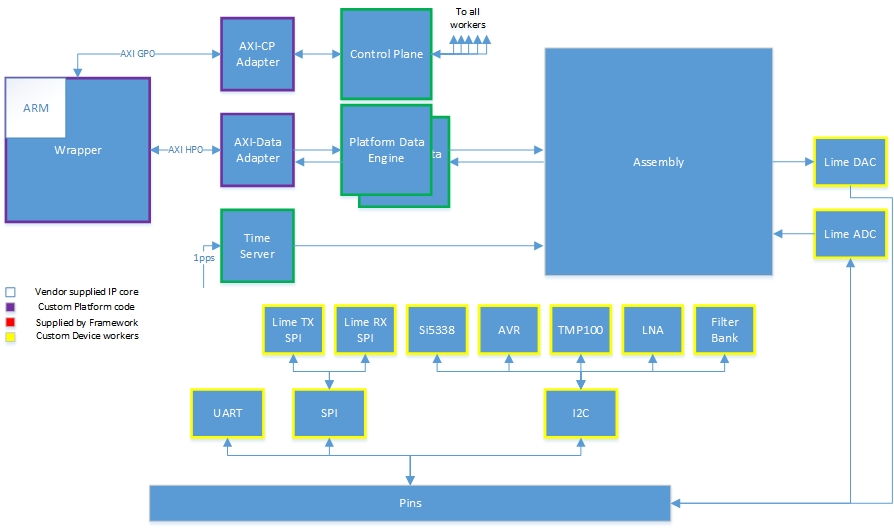
\includegraphics[scale=0.65]{matchstiq_BSP_toplevel}}
      \caption{Top Level Block Diagram}
      \label{fig:toplevel}
    \end{figure}

\pagebreak
\noindent The block diagram in Figure \ref{fig:workerlevel} shows the connectivity between device and proxy workers in support of the Matchstiq-Z1's OpenCPI BSP.
    \begin{figure}[H]
      \centerline{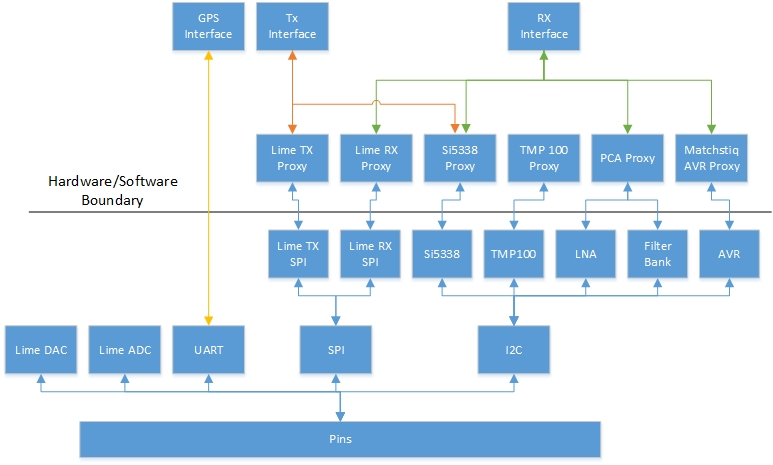
\includegraphics[scale=0.65]{matchstiq_BSP_worker}}
      \caption{Workers Block Diagram}
      \label{fig:workerlevel}
    \end{figure}

\section{Petalinux}
  \textbf{NOTE: The method of forcing an OpenCPI supported Linux OS and compiler onto a platform is no longer the recommended method for enabling a new GPP platform. The new recommended method is to enable OpenCPI for the existing platform's OS by integrating the cross compiler tools supplied by the vendor, when applicable.} \\

\noindent The first task that needs to be completed is to install the OpenCPI version of Petalinux onto the platform.  In order to boot the platform on the Matchstiq-Z1, there are three things that are needed on the SD card: Device tree, Linux kernel, and the root filesystem.  The First Stage Boot Loader for the Matchstiq is located in flash and was left alone for our implementation.\\

\noindent There are environment variables that U-Boot (second stage boot loader) use to load files from the SD card into memory to boot the processor.  The original Matchstiq-Z1 SD card image had created a kernel with a small root file system embedded within the kernel. This used different U-boot settings and we had to edit these settings to boot our version. On the Matchstiq-Z1, these U-Boot variables are located on the second partition of the SD card. This is important to keep in mind when trying to create new SD cards for the Matchstiq-Z1. \\

\noindent To enable the MatchStiq-Z1 to support the OpenCPI \textit{Network Mode} development environoment, an Ethernet connection was required.  While the Matchstiq-Z1 does not have an Ethernet port,  a USB to Ethernet adapter and a modification to the Petalinux kernel were all that was needed to enable Ethernet for this platform. It is worth noting that the Zedboard device tree/build was also modified to support USB on-the-go.

\section{Cross Compiler}

When the Matchstiq-Z1 was being brought into the framework, the Zedboard platform work had already integrated the cross compiler for Zynq-7000 into OpenCPI.  Had this not been the case there would need to be work done to integrate a cross compiler into the framework.

\section{Device Workers}
The platform has a set of devices that are connected to the FPGA.  The devices were analyzed for functionality and each function was implemented as a device worker. As is the case with component reuse, several of the device workers were already available (lime\_spi, lime\_tx, lime\_rx, lime\_dac, lime\_adc), since they had been previously developed in support of the ZedBoard/Zipper SDR. However, some of these device workers did require expanding their support for a different clock distribution circuit compared to that of the Zedboard/Zipper SDR.

  \subsection{I2C Bus}
  There are several devices connected to the I2C bus, the peripherals and their slave addresses were known from the Epiq documentation.  The order and the values of the register settings were determined by monitoring the I2C bus with a bus analyzer while using Epiq's provided API.\\

\noindent The I2C connected devices are: SI5338 clock generator, TMP100 temperature sensor, AVR microcontroller, a low noise amplifier, and a RF filter bank.  A device worker and a  proxy worker was developed for each of these peripherals.

  \subsection{SPI Bus}
    There is a single slave SPI connection on the Matchstiq-Z1 platform connecting to the LMS6002D transceiver for control to the configuration registers of the transceiver.  A device worker and a device proxy needed to be implemented for this device, this was reused from the Zedboard platform.

  \subsection{DAC/ADC}
    There are 12 bit D/A and A/D data lines to move the I/Q samples between the LMS6002D and FPGA.  Device workers that were developed for the Zedboard/Zipper SDR were reused, with modifications to the clock distribution.

  \subsection{TX/RX}
    There are TX and RX enable pins and registers to enable/disable the RF portions of the transceiver.  Device workers and proxies that were developed for the Zedboard/Zipper SDR were reused but only supported access to the tx/rx enable/disable pins of the transceiver, where as the Matchstiq-Z1 does not provide direct access to those pins. Therefore, these device workers and proxies were modified to support enable/disable of the transceiver's RF transmitter via a register.

  \subsection{GPS UART}
    There is a GPS receiver on the Matchstiq-Z1 that communicates with the FPGA over UART.  A device worker and a device proxy (TBD) needed to be implemented for this device.

\section{HDL Platform}
  The device workers that are described above are instantiated in the container.  The ARM processing system needed to be instantiated into the platform and configured in the correct way. This was a non trivial task to learn how to do but was reused from the Zedboard platform.

  \subsection{Control Plane Integration}
    The control plane modules are connected to General Purpose AXI port 0 on the ARM processor.  An adapter needed to be written to take data being streamed to the FPGA via AXI to be passed to the HDL framework.  Driver software also needed to be written for the processor to move data from the ARM processor down to the FPGA.  This driver was reused from the Zedboard platform.


  \subsection{Data Plane Integration}
    The data plane modules are connected to a High performance AXI port on the ARM processor.  An adapter needed to be written to take data being streamed to the FPGA via AXI to be passed to the HDL framework.  Driver software also needed to be written for the processor to move data from the ARM processor down to the FPGA.  This driver was reused from the Zedboard platform.

\section{Common interfaces}
  Each radio platform will have a common generic software interface for receive and transmit.  These interfaces are documented in the workers data sheets.  The workers for each of these interfaces needed to be implemented on the Matchstiq-Z1 platform.

\end{document}
